\section{Moment.js}

A második mélyebben megvizsgált kódbázis a moment.js\footnote{https://momentjs.com/} lesz. A moment éveken át volt a de facto JavaScript-ben írt dátum-idő könyvtár, azonban 2020-ban különböző okoknál fogva a fejlesztése befejeződött.

A moment kódbázisa két szempontból lesz érdekes: egyrészt "késznek" tekinthető, másrészt egy nagyon jól definiált, kis problémát volt hivatott megoldani a kezdetekből.

Ideális esetben a legelső kiadástól lenne érdemes kezdeni az analízist, azonban a moment 1.0 megjelenésekor sem unit tesztek, sem coverage report nem voltak a projekthez, ráadásul a kódbázis egy masszív JavaScript fájl volt. A moment 2.0 megjelenése azonban viszonylag közel van az 1.0-hoz és a 2.10.5-ös minor release-től kezdve elérhető a coverage report, úgyhogy az lesz a kezdőpont

A \ref{fig:moment-2.10.5-changes} ábrán látható az összes fájl módosítási száma és a fájlokhoz tartozó egyedi szerzők száma. Egy érdekes dolog már most megfigyelhető: ellentétben a vue-val, itt a szórás a különböző fájlok módosítási számai között viszonylag alacsony. Ehhez viszont hozzátartozik a korábban említett 1.0-ás kiadás, ahol a kódbázis egy \code{moment.js} nevű fájl volt, aminek a története egy újraírás miatt nem jelenik meg a 2.x-es kiadásokban. 

\begin{figure}[H]
    \centering
    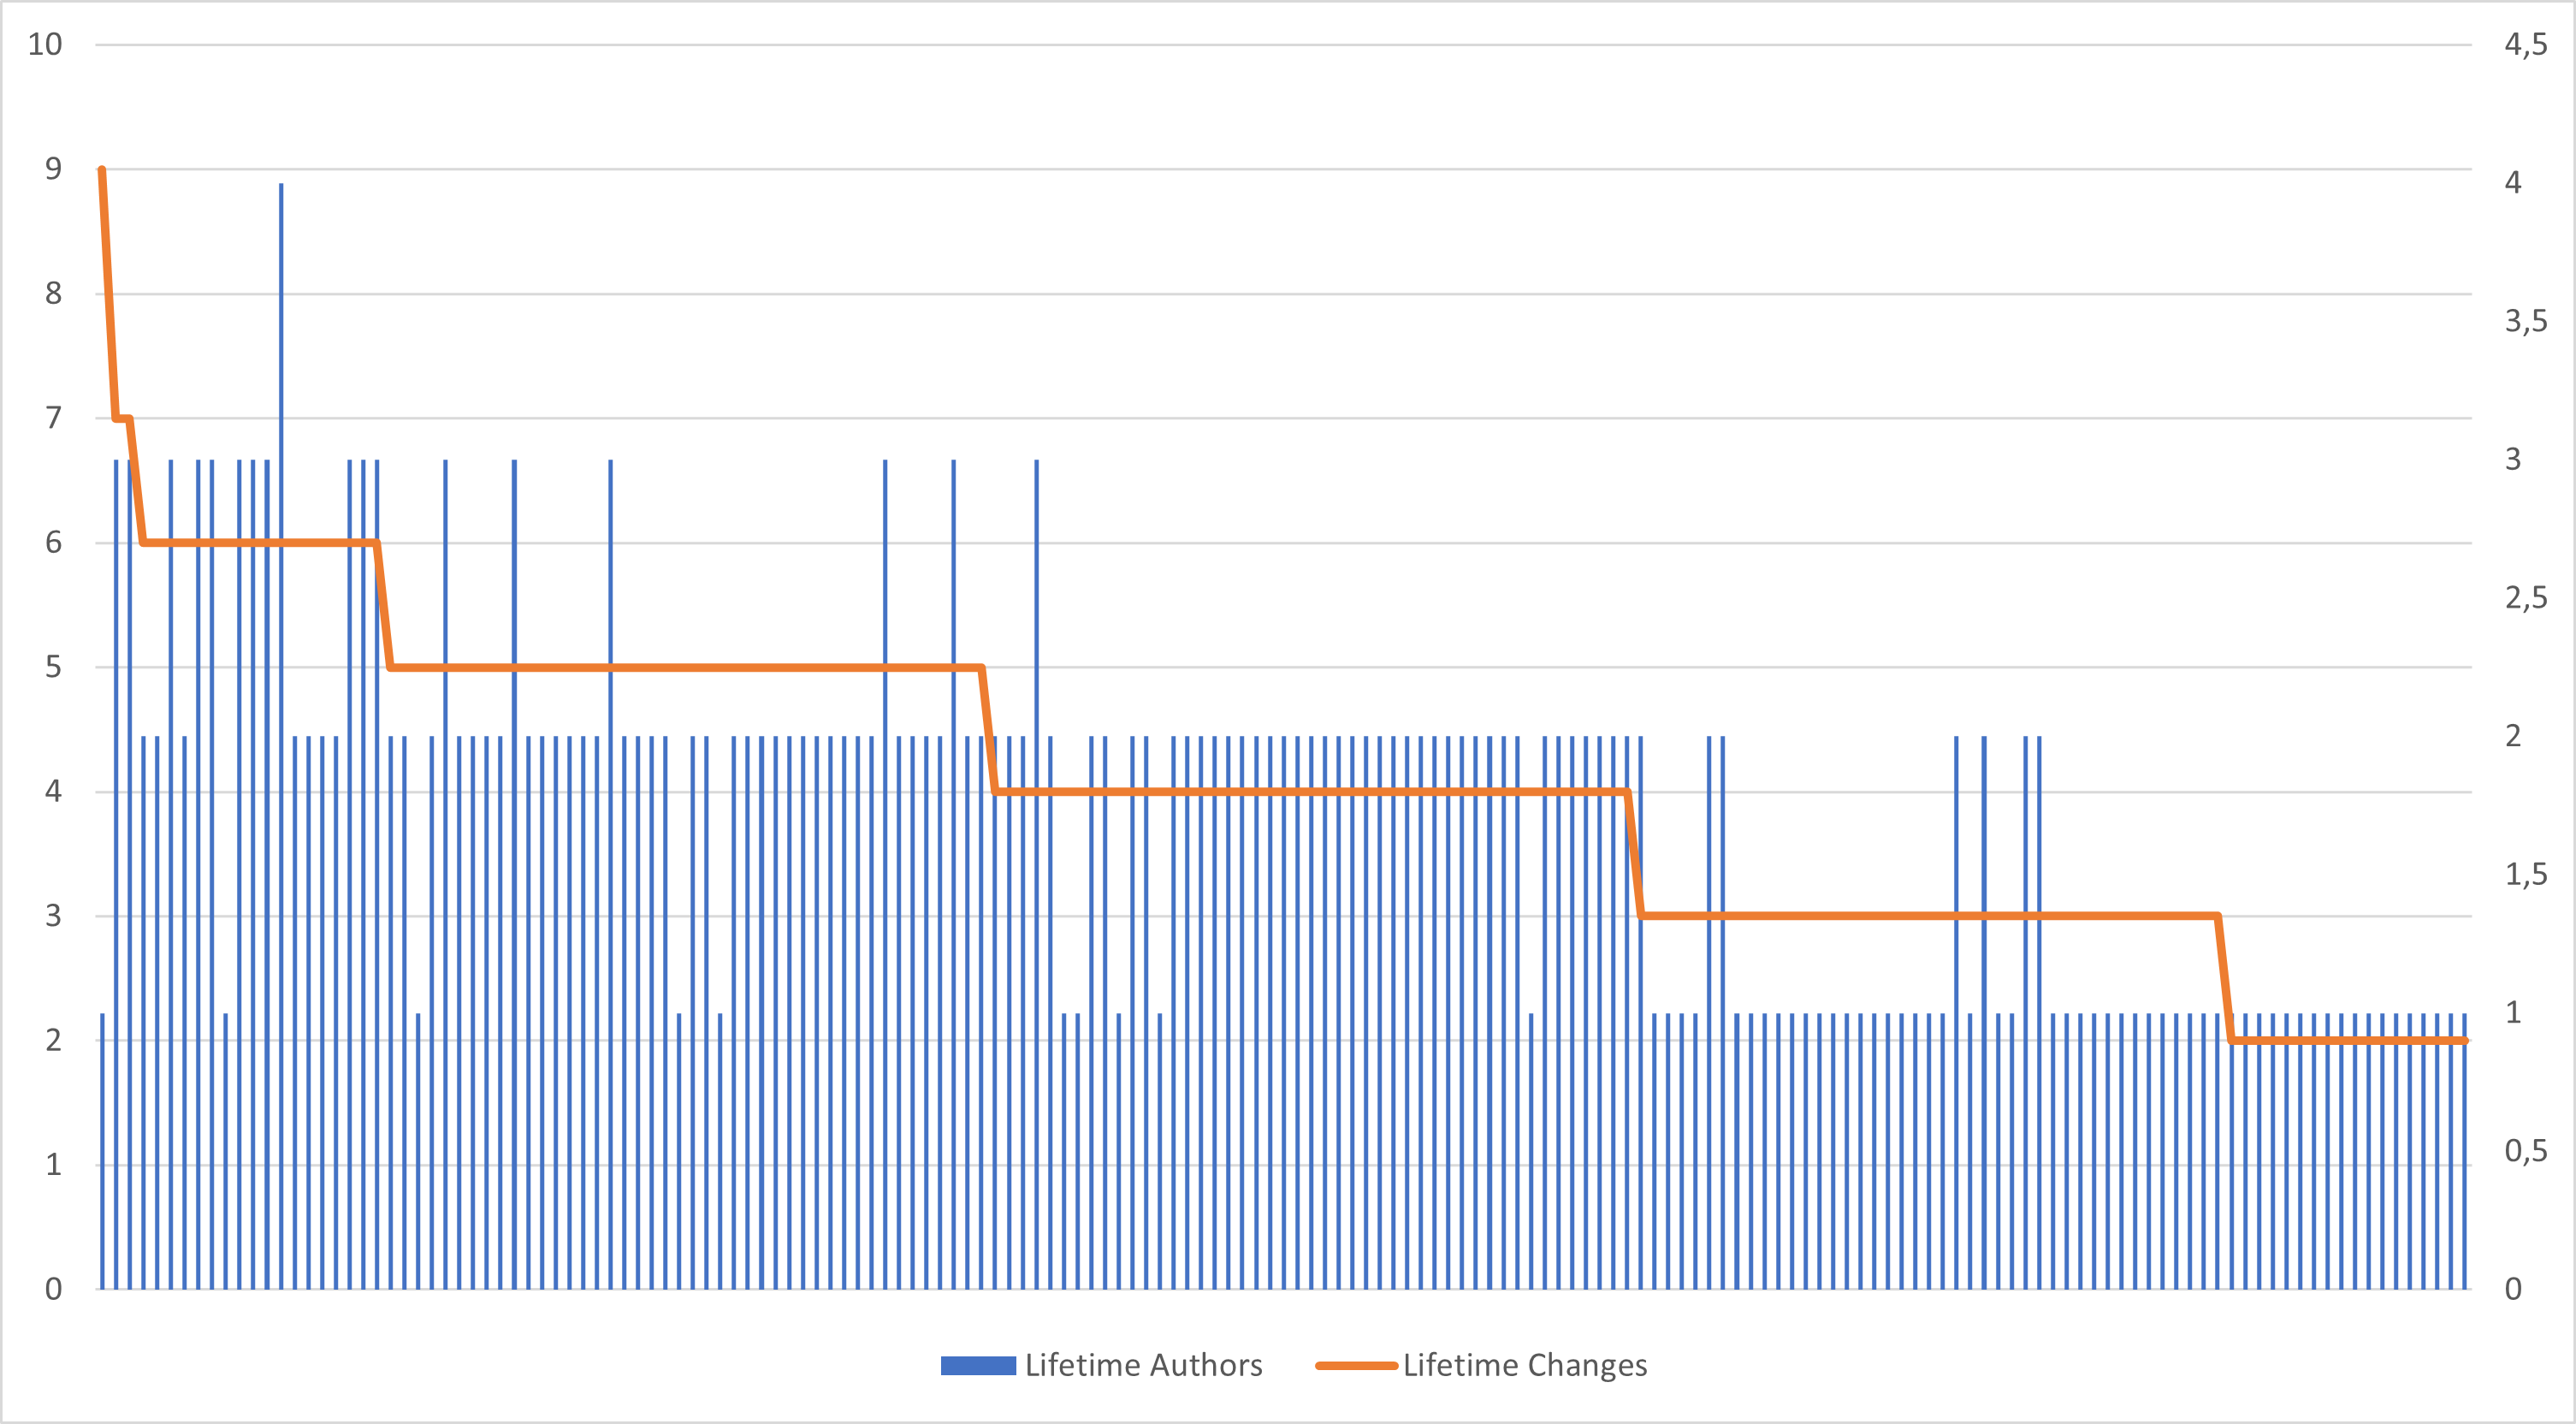
\includegraphics[width=1\textwidth]{images/moment/moment-2.10.5-changes.png}
    \caption{Moment.js 2.10.5-ös kiadásában lévő fájlok módosítási számai}
    \label{fig:moment-2.10.5-changes}
\end{figure}

A \ref{fig:moment-2.10.5-hist} ábrán látható hisztogram jól demonstrálja a kódbázis állapotát a 2.10.5-ös kiadásban. Ugyan technikailag itt is látható az a trend, hogy a fájlok túlnyomó többsége módosítások számát tekintve az alsó 40\%-ban van, azonban itt ez csalóka, hiszen az módosítások számának intervalluma csak 1-től 9-ig terjed.

\begin{figure}[H]
    \centering
    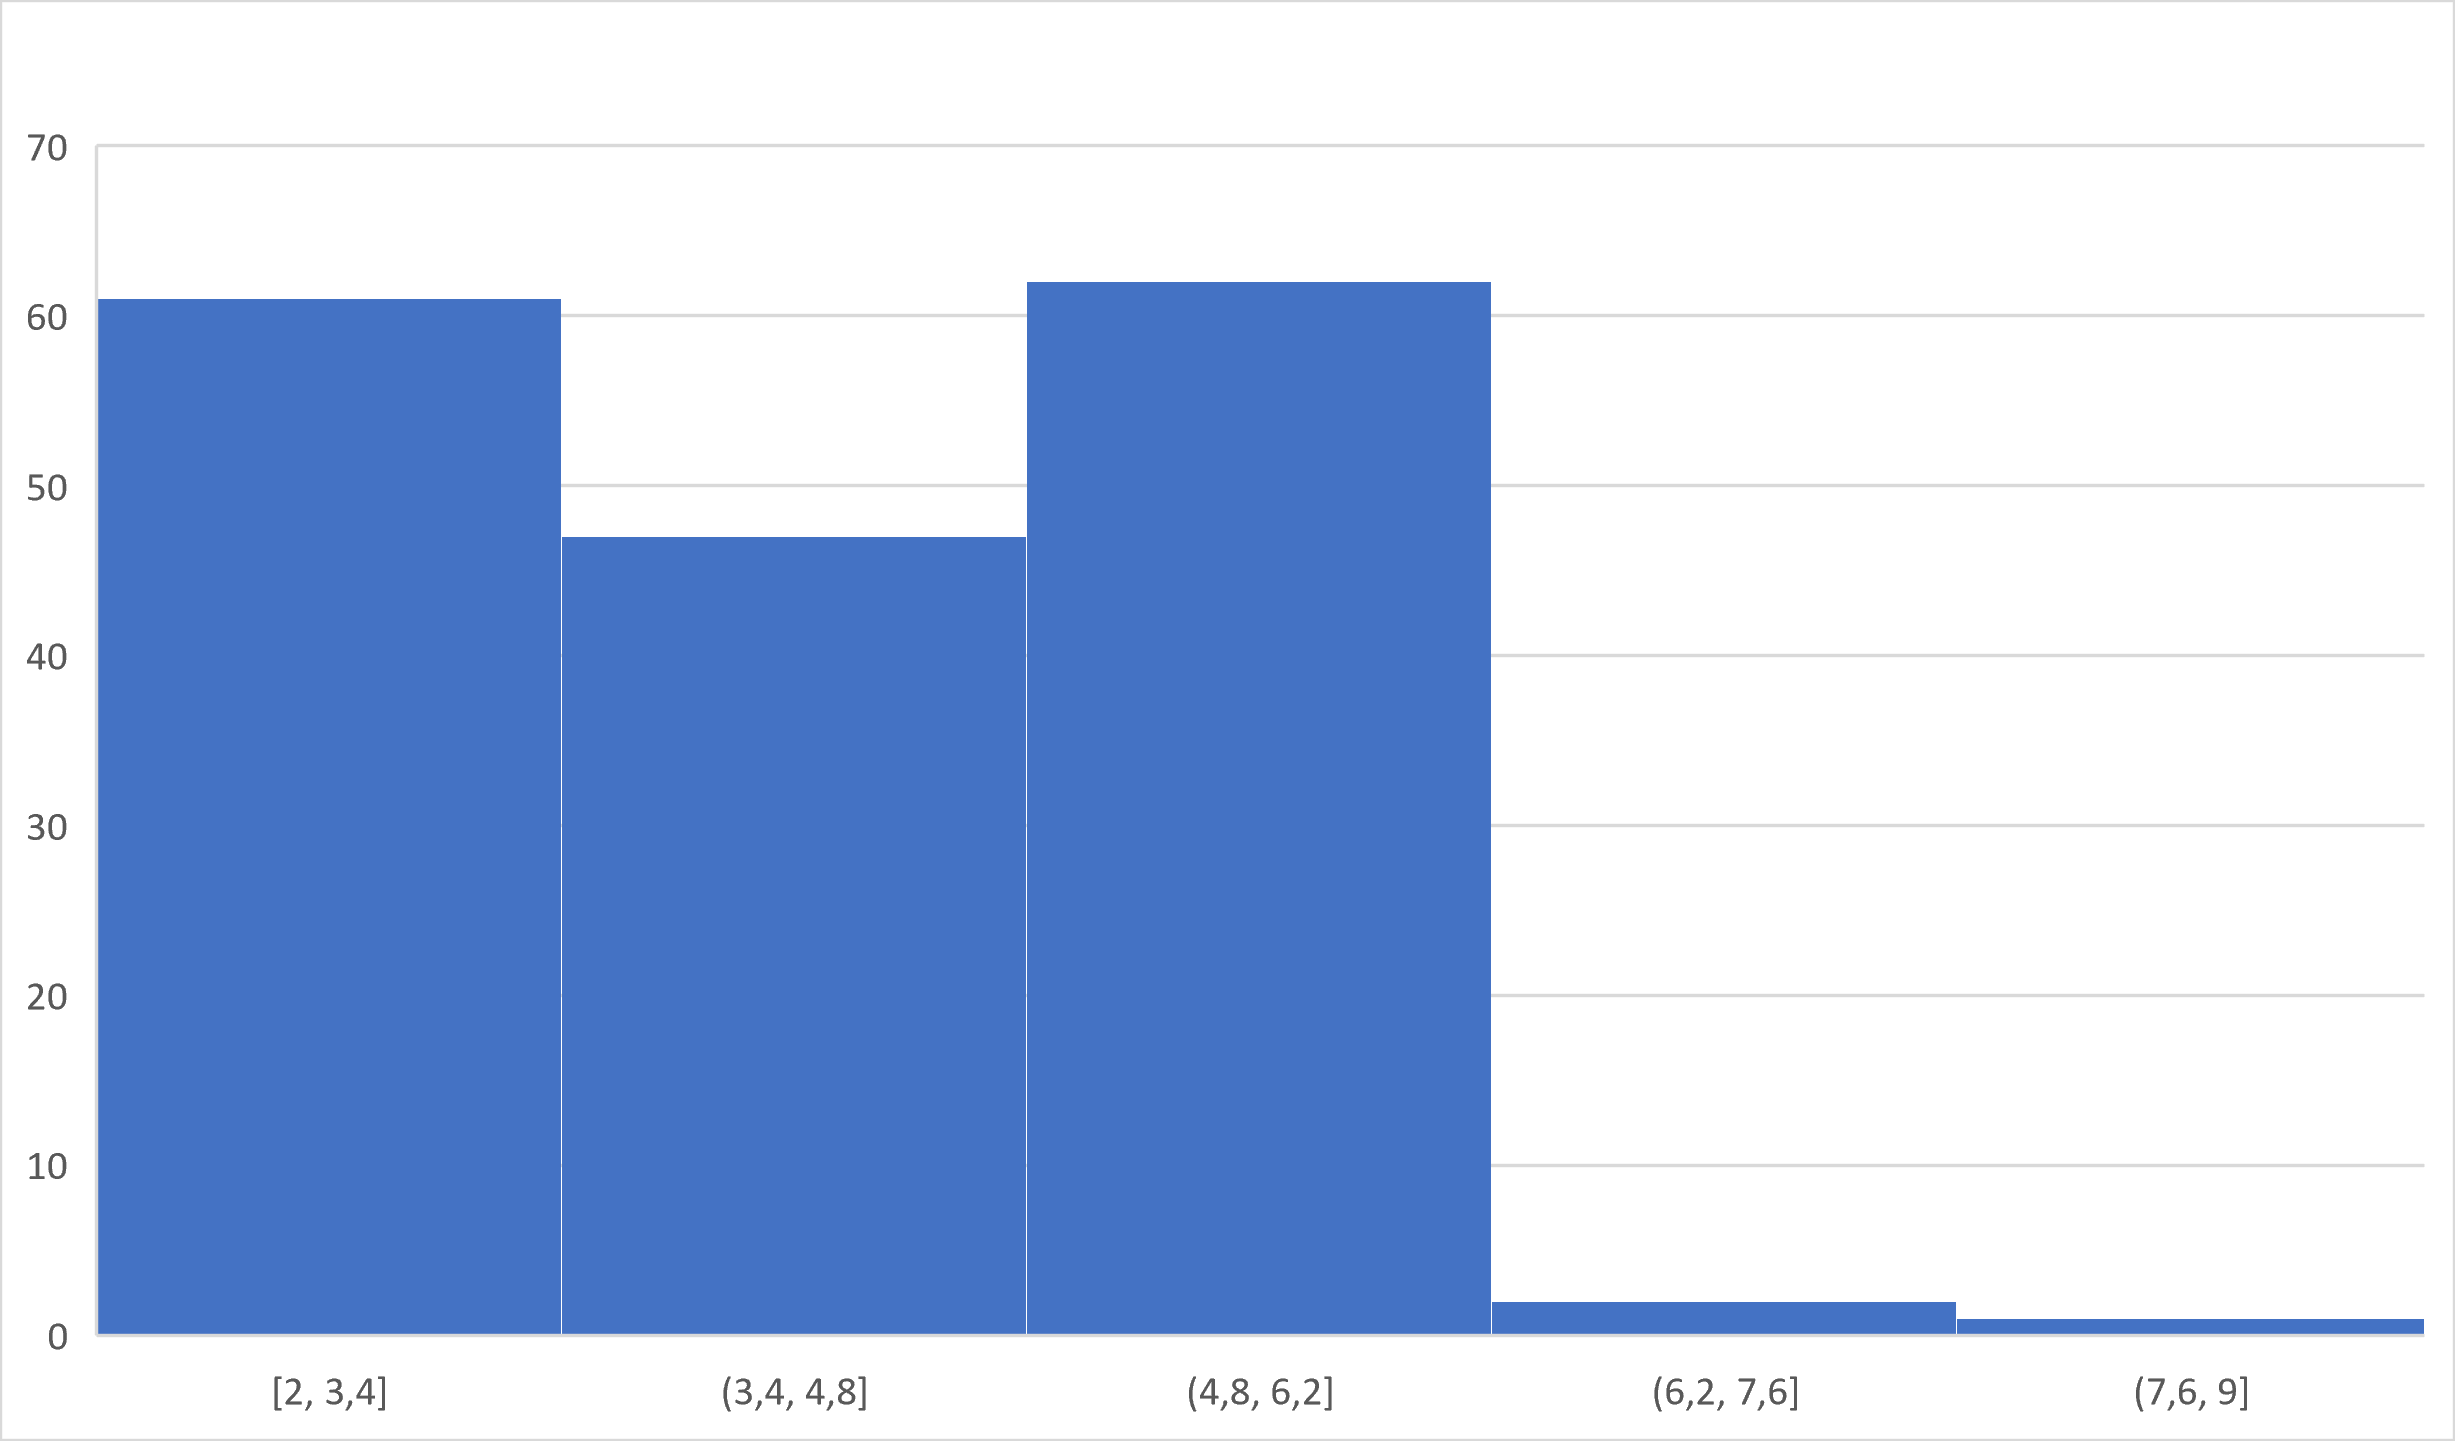
\includegraphics[width=1\textwidth]{images/moment/moment-2.10.5-hist.png}
    \caption{Moment.js 2.10.5-ös kiadásában lévő fájlok módosítási számainak hisztogramja}
    \label{fig:moment-2.10.5-hist}
\end{figure}

Ugorjunk az időben a 2.20.5-ös verzióhoz tartozó snapshot-ra. A \ref{fig:moment-2.20.5-changes} ábra már sokkal jobban hasonlít a vue-nál látottakhoz: változtatások számának tekintetében 

\begin{figure}[H]
    \centering
    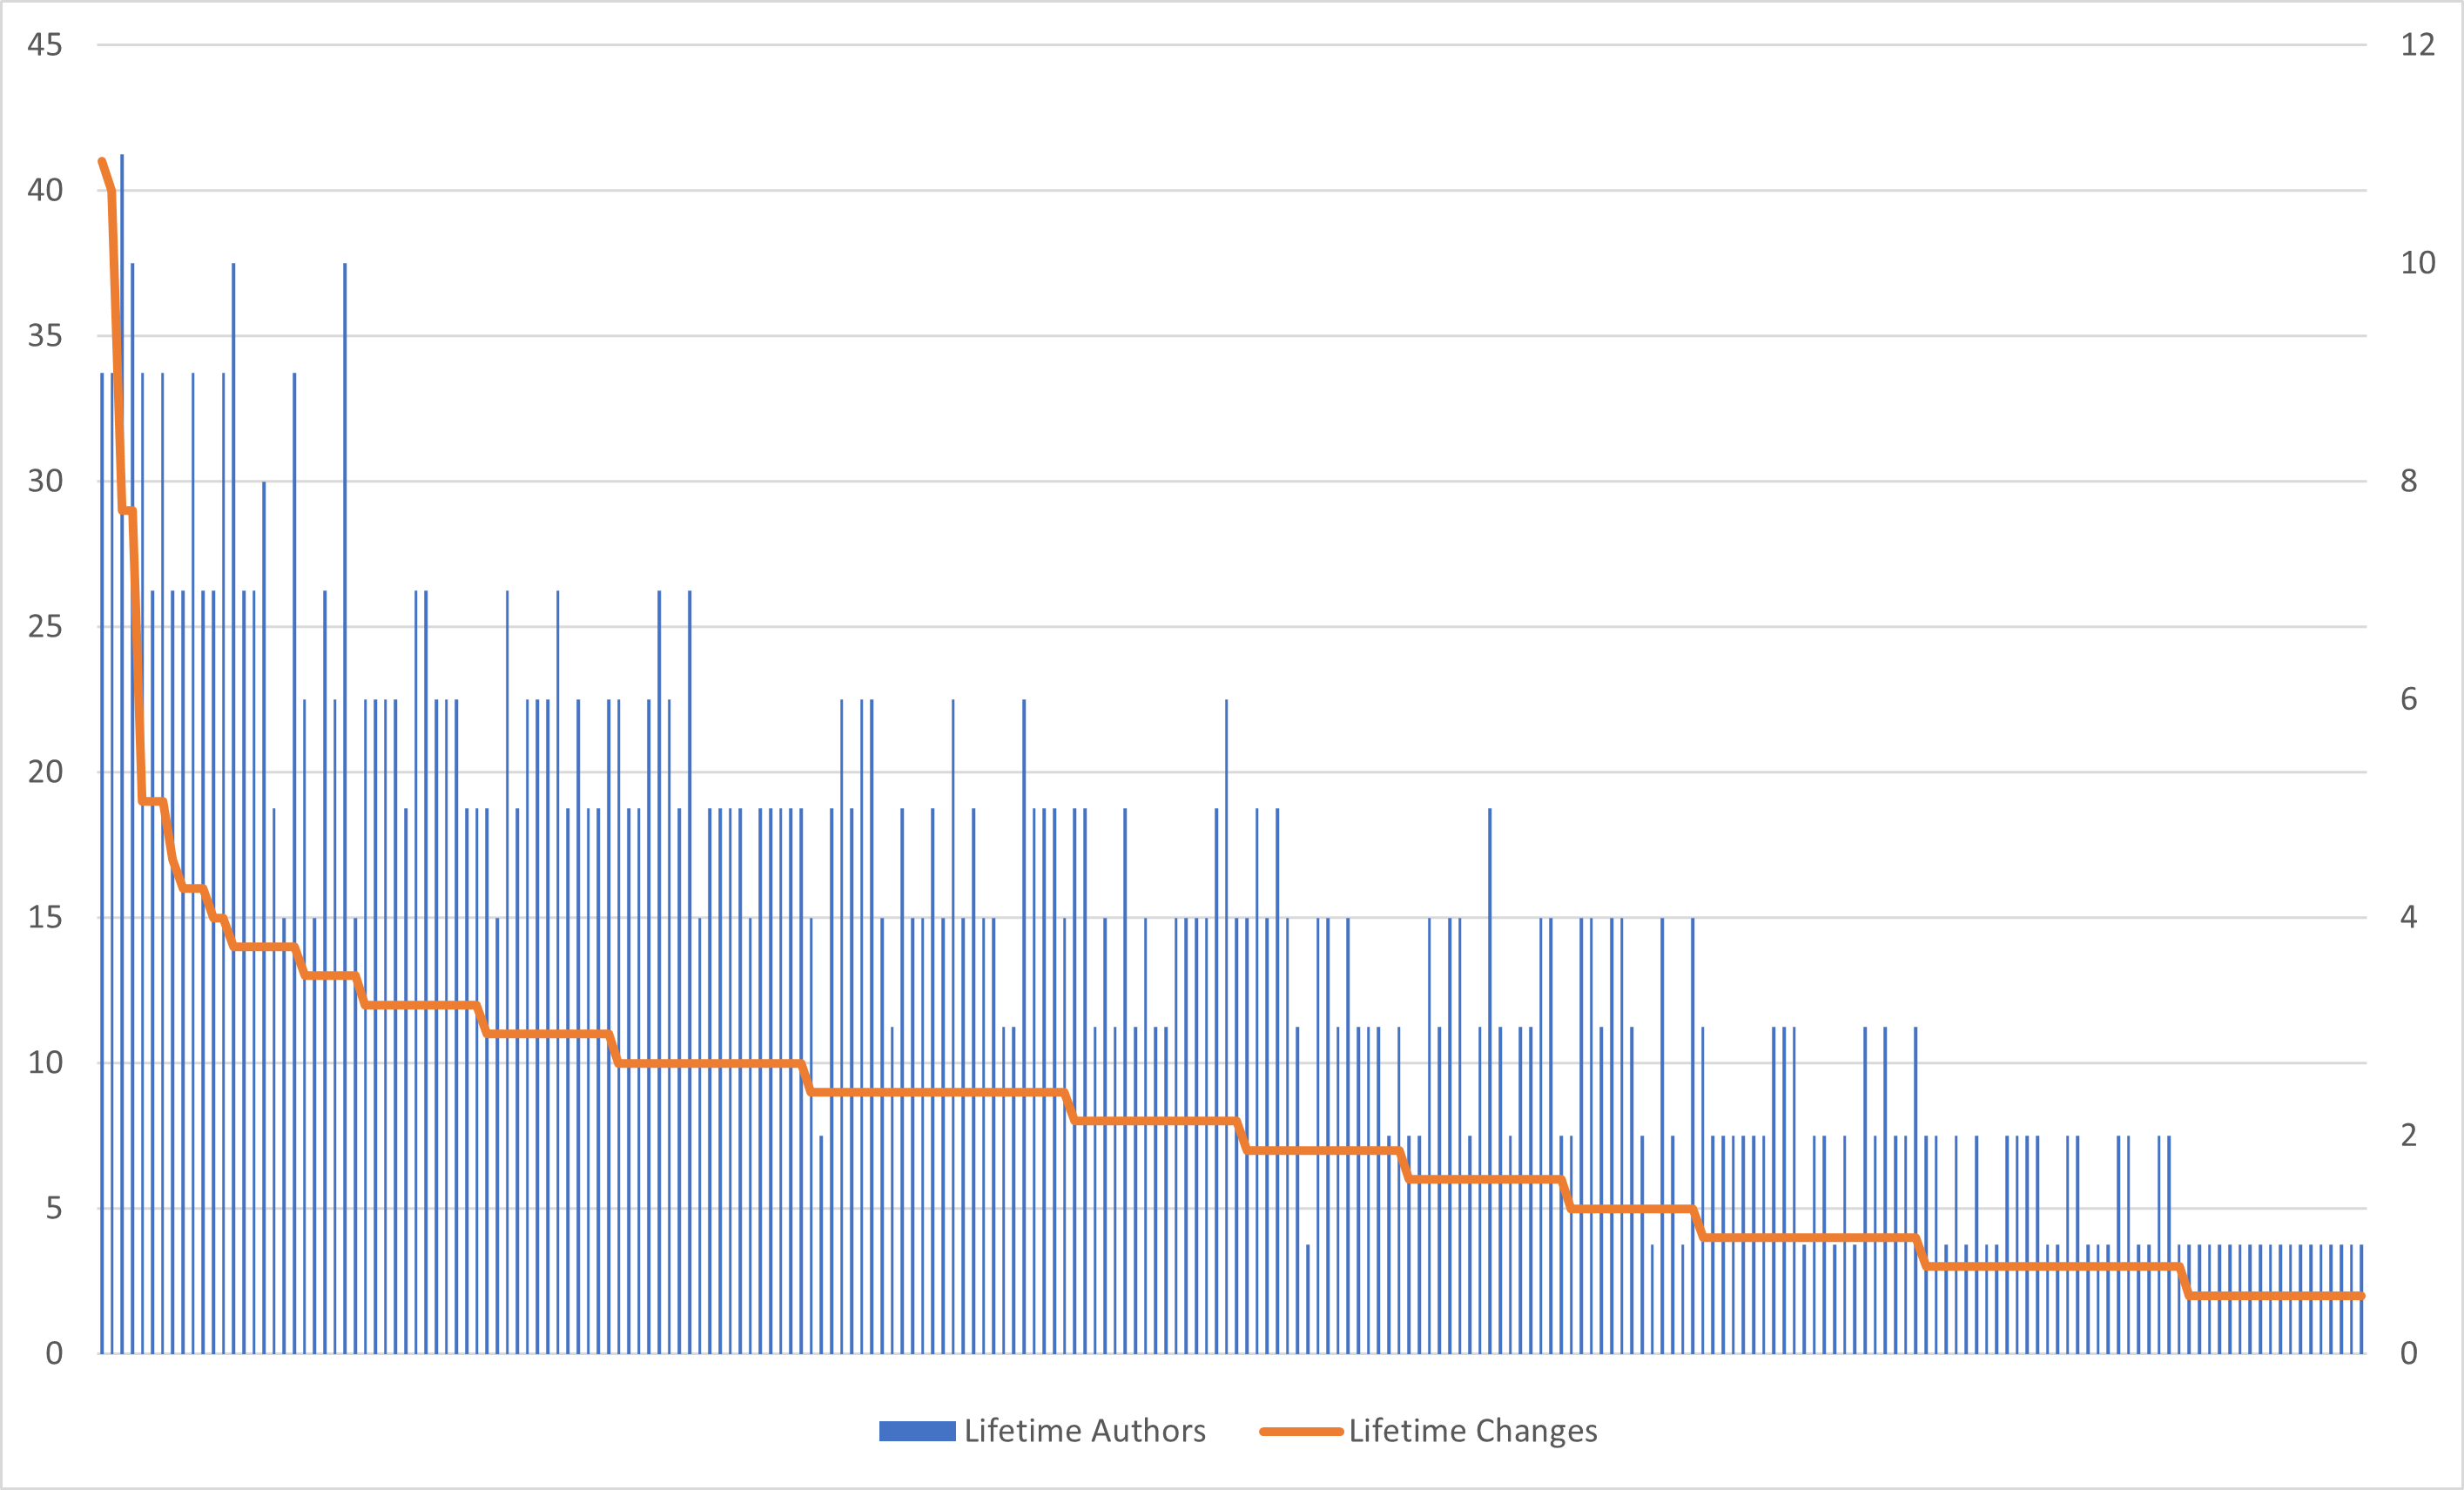
\includegraphics[width=1\textwidth]{images/moment/moment-2.20.5-changes.png}
    \caption{Moment}
    \label{fig:moment-2.20.5-changes}
\end{figure}

\begin{figure}[H]
    \centering
    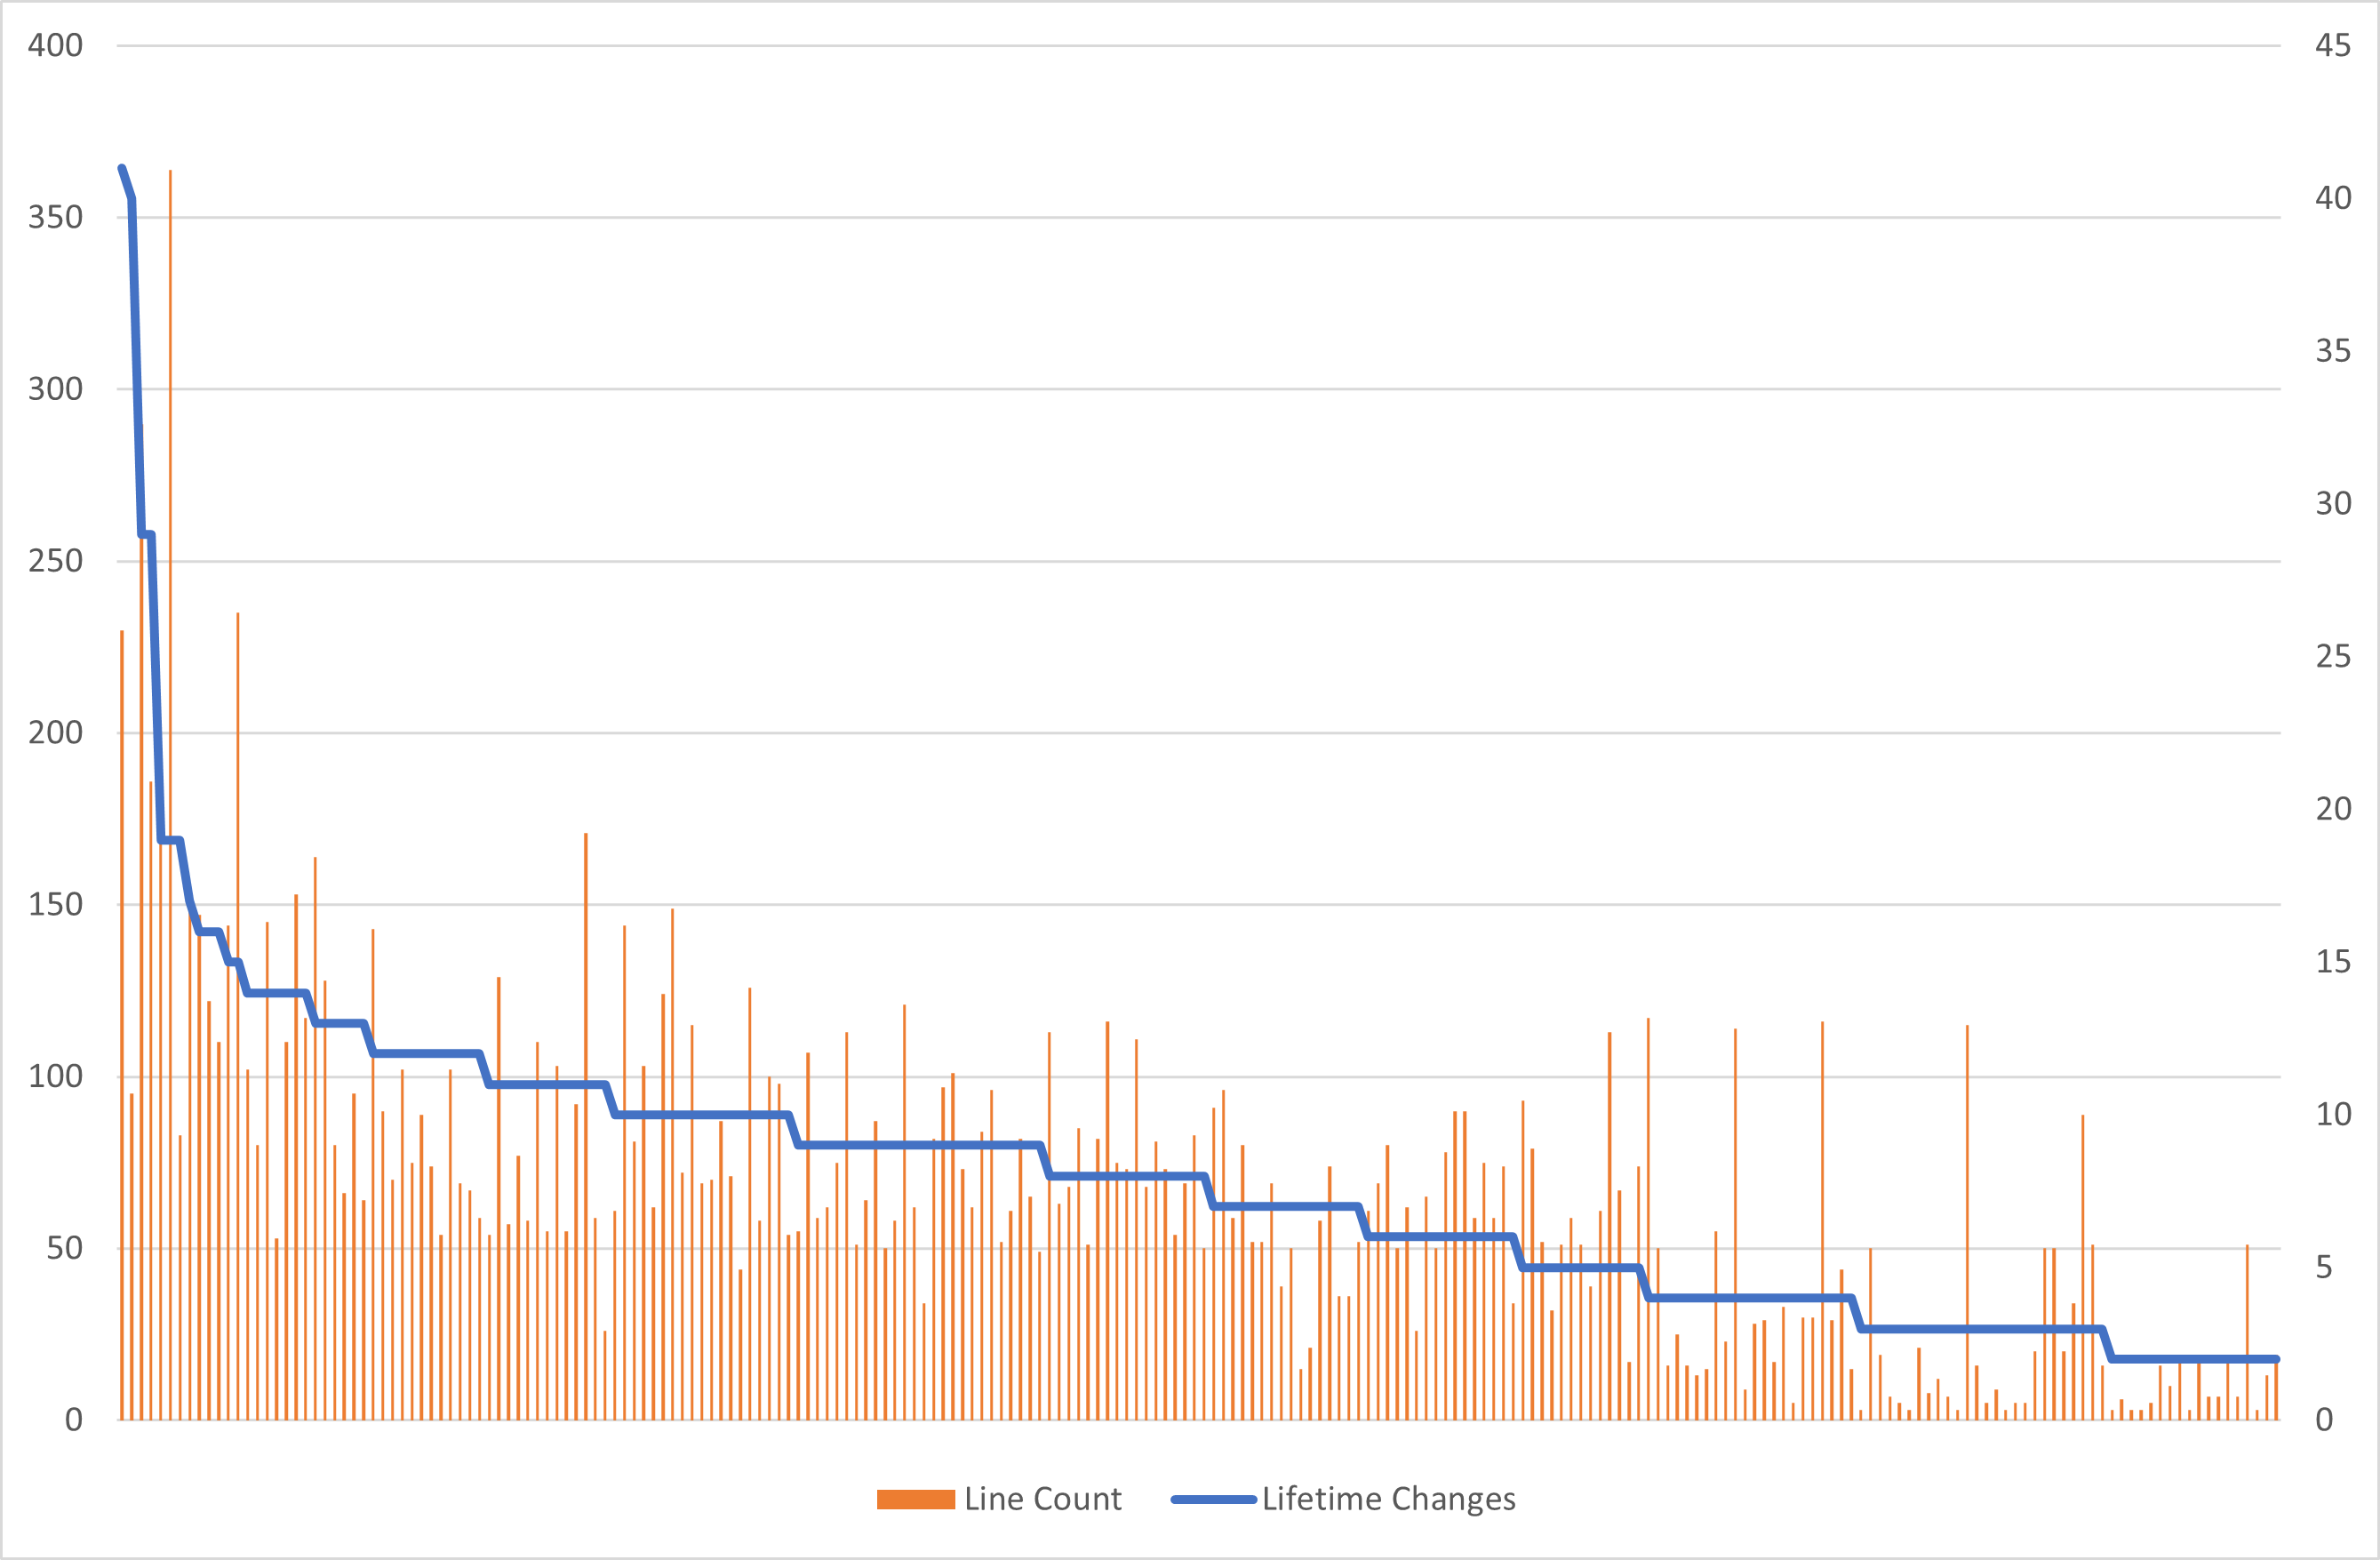
\includegraphics[width=1\textwidth]{images/moment/moment-2.20.5-auth.png}
    \caption{Moment}
    \label{fig:moment-2.20.5-auth}
\end{figure}

\begin{figure}[H]
    \centering
    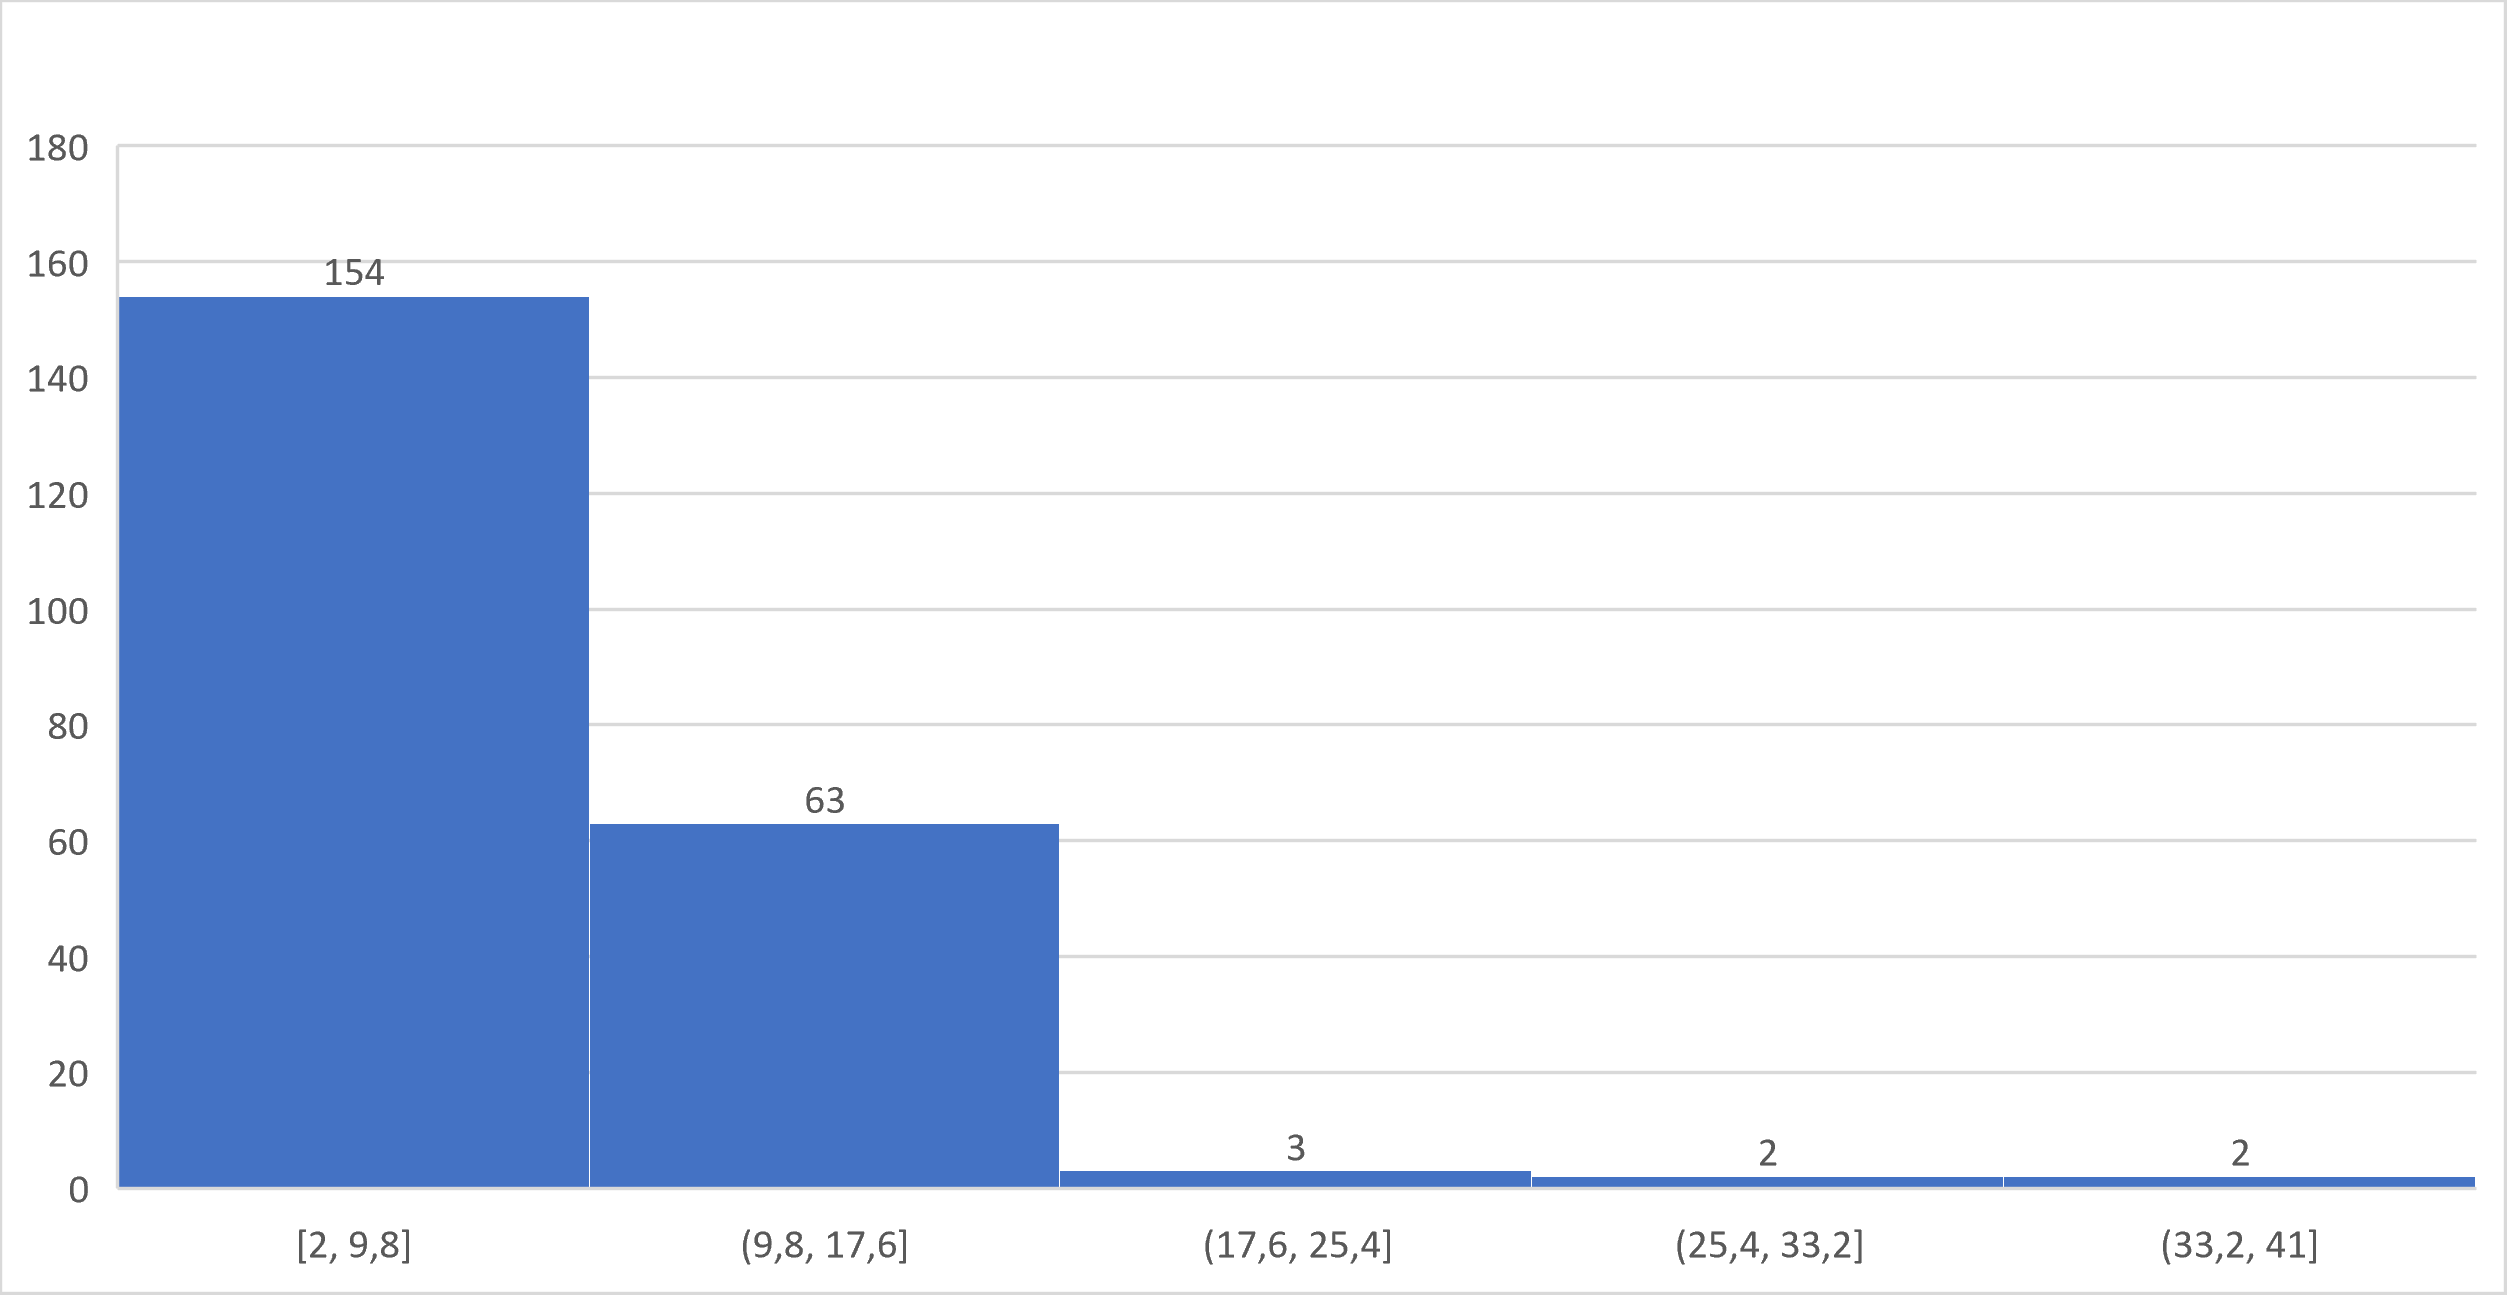
\includegraphics[width=1\textwidth]{images/moment/moment-2.20.5-hist.png}
    \caption{Moment}
    \label{fig:moment-2.20.5-hist}
\end{figure}


\begin{figure}[H]
    \centering
    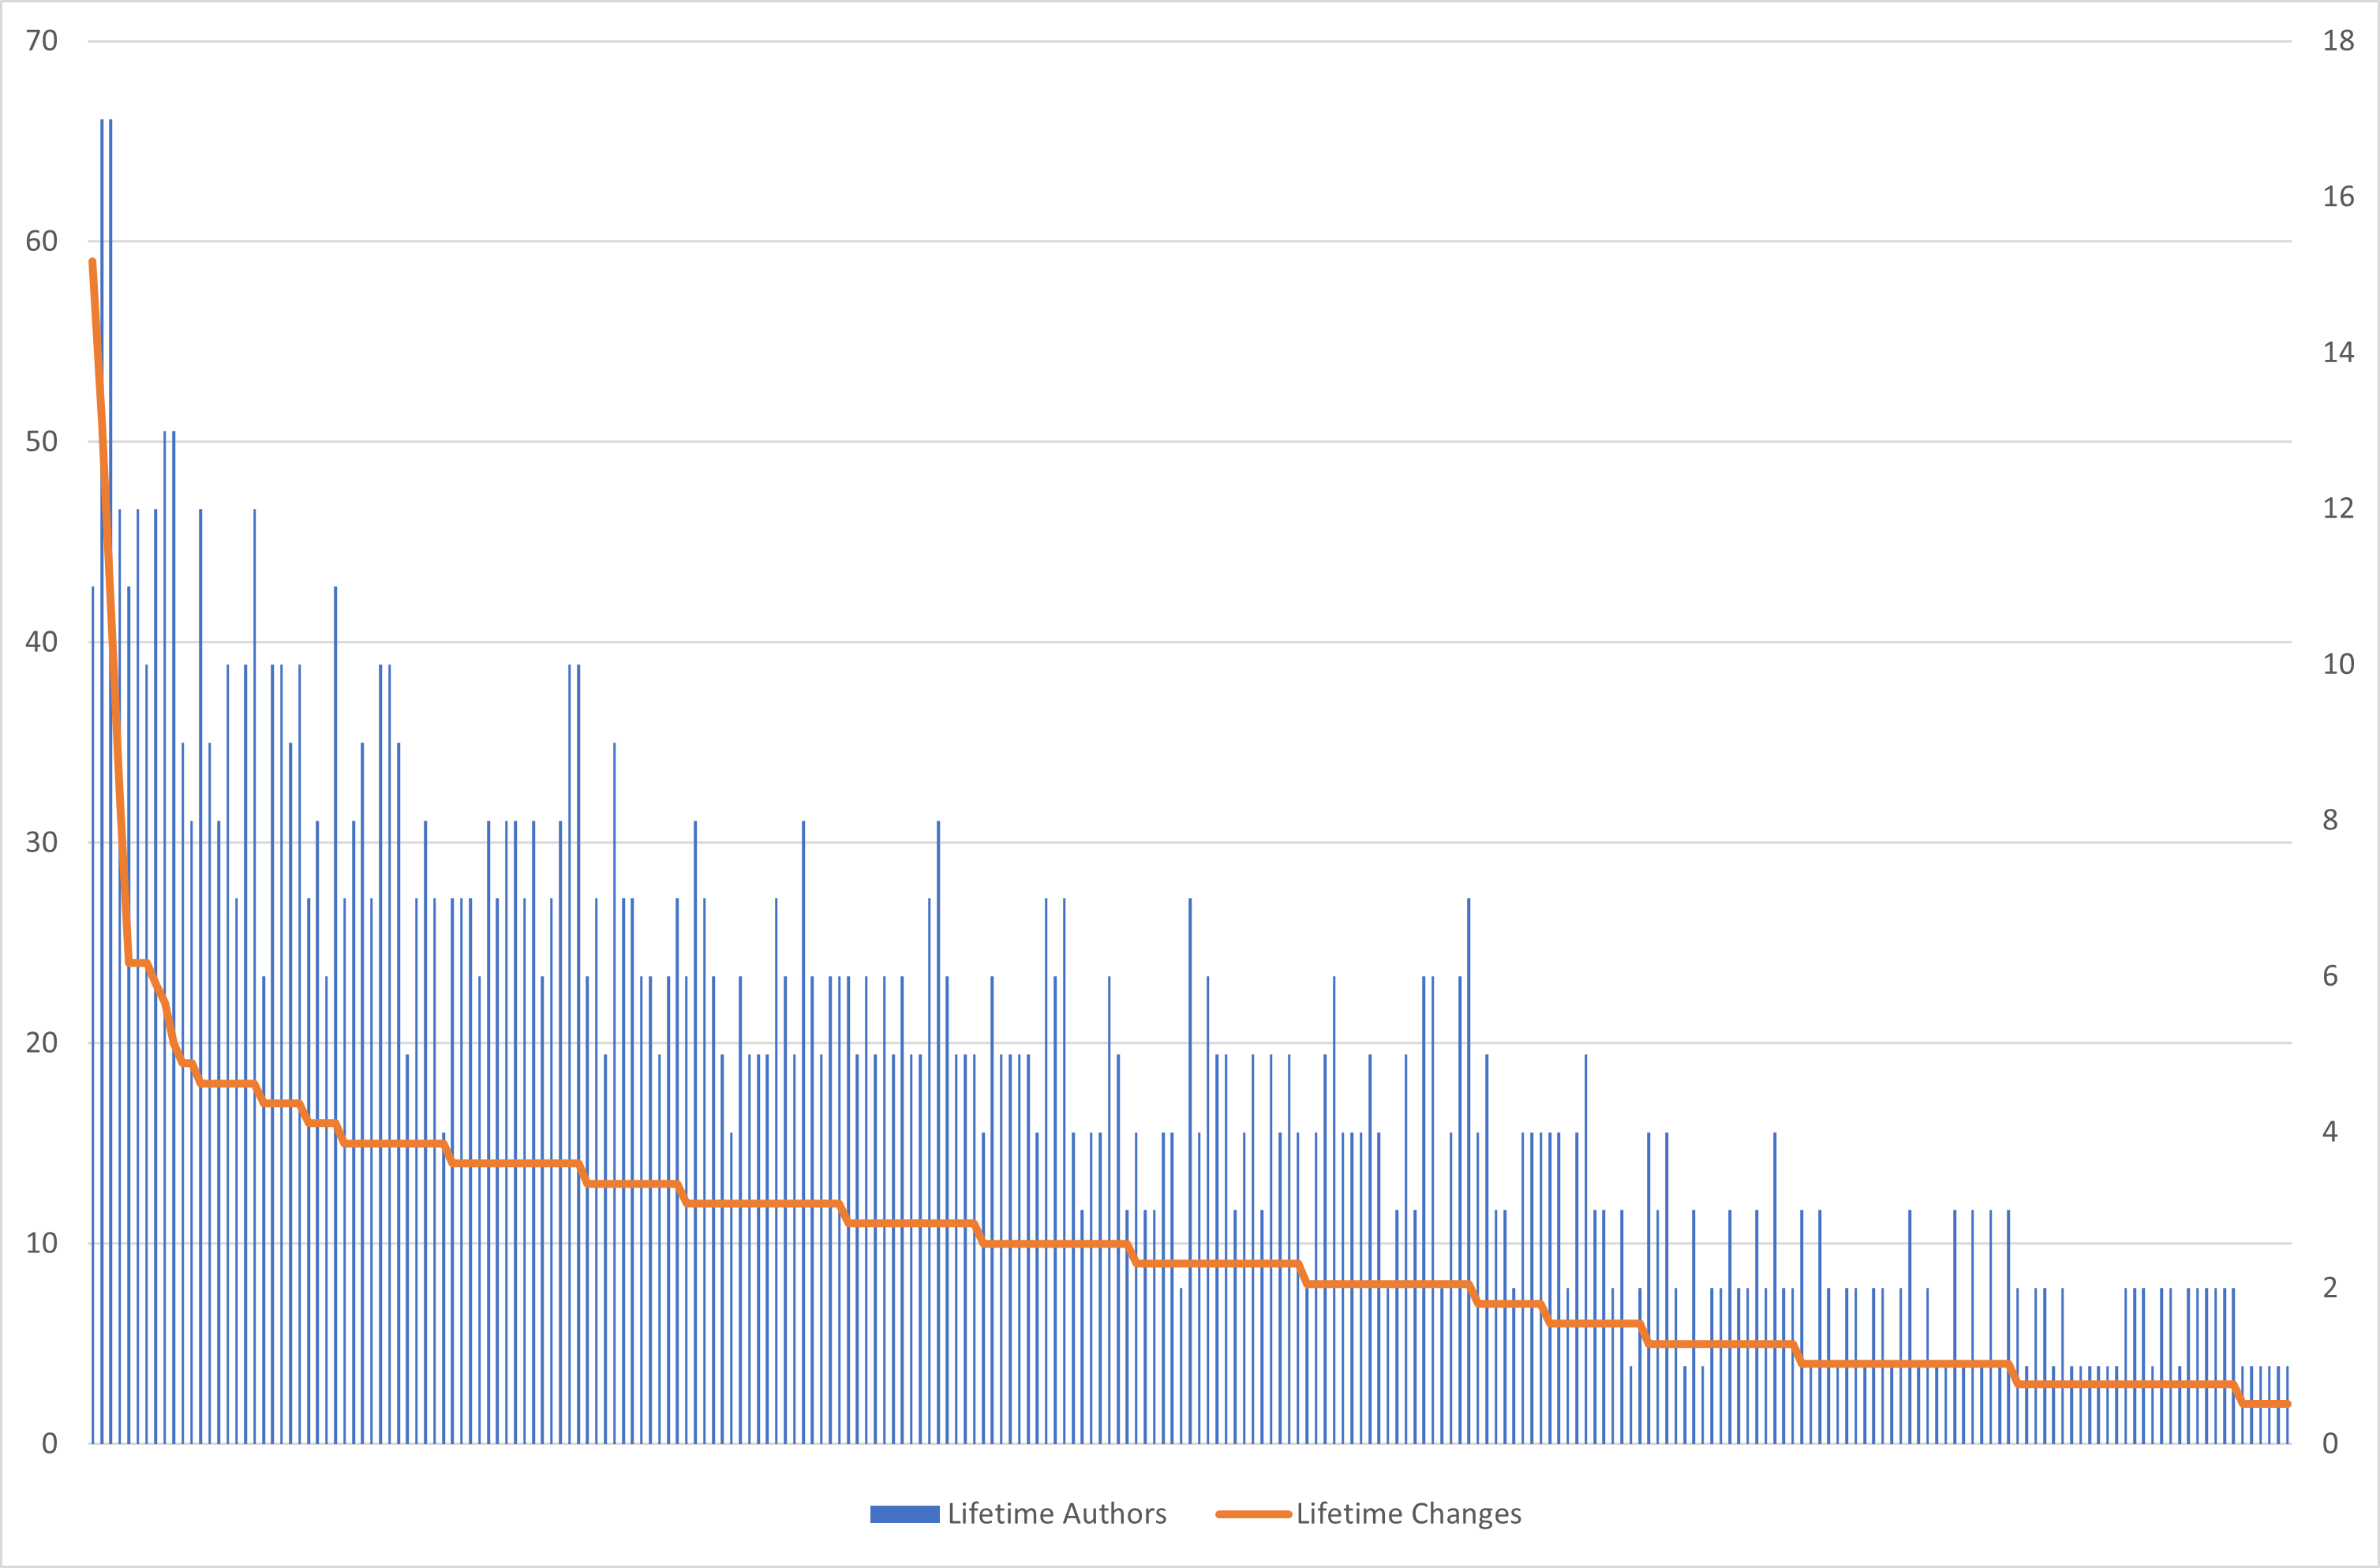
\includegraphics[width=1\textwidth]{images/moment/moment-dev-changes.png}
    \caption{Moment}
    \label{fig:moment-2.10.5-changes}
\end{figure}

\begin{figure}[H]
    \centering
    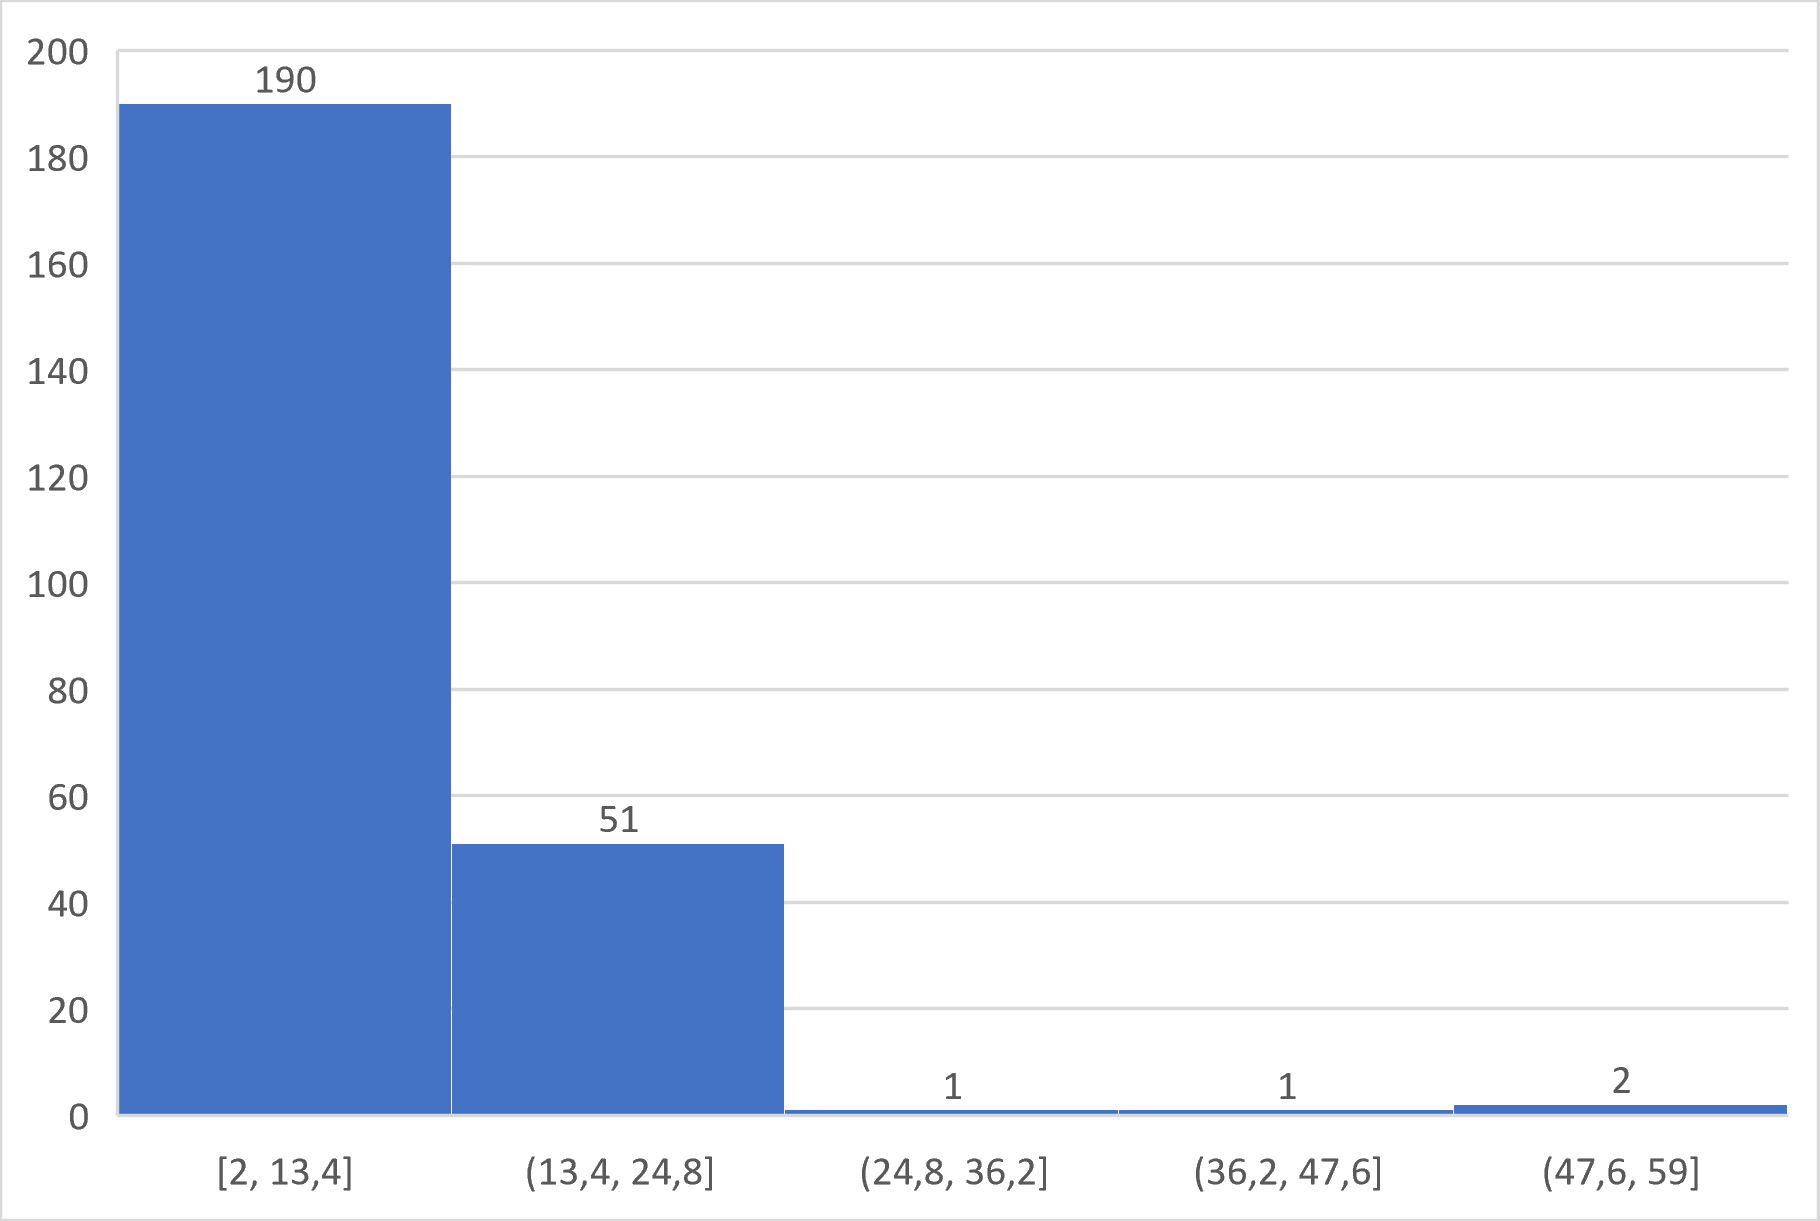
\includegraphics[width=1\textwidth]{images/moment/moment-dev-hist.png}
    \caption{Moment}
    \label{fig:moment-2.10.5-changes}
\end{figure}

\begin{figure}[H]
    \centering
    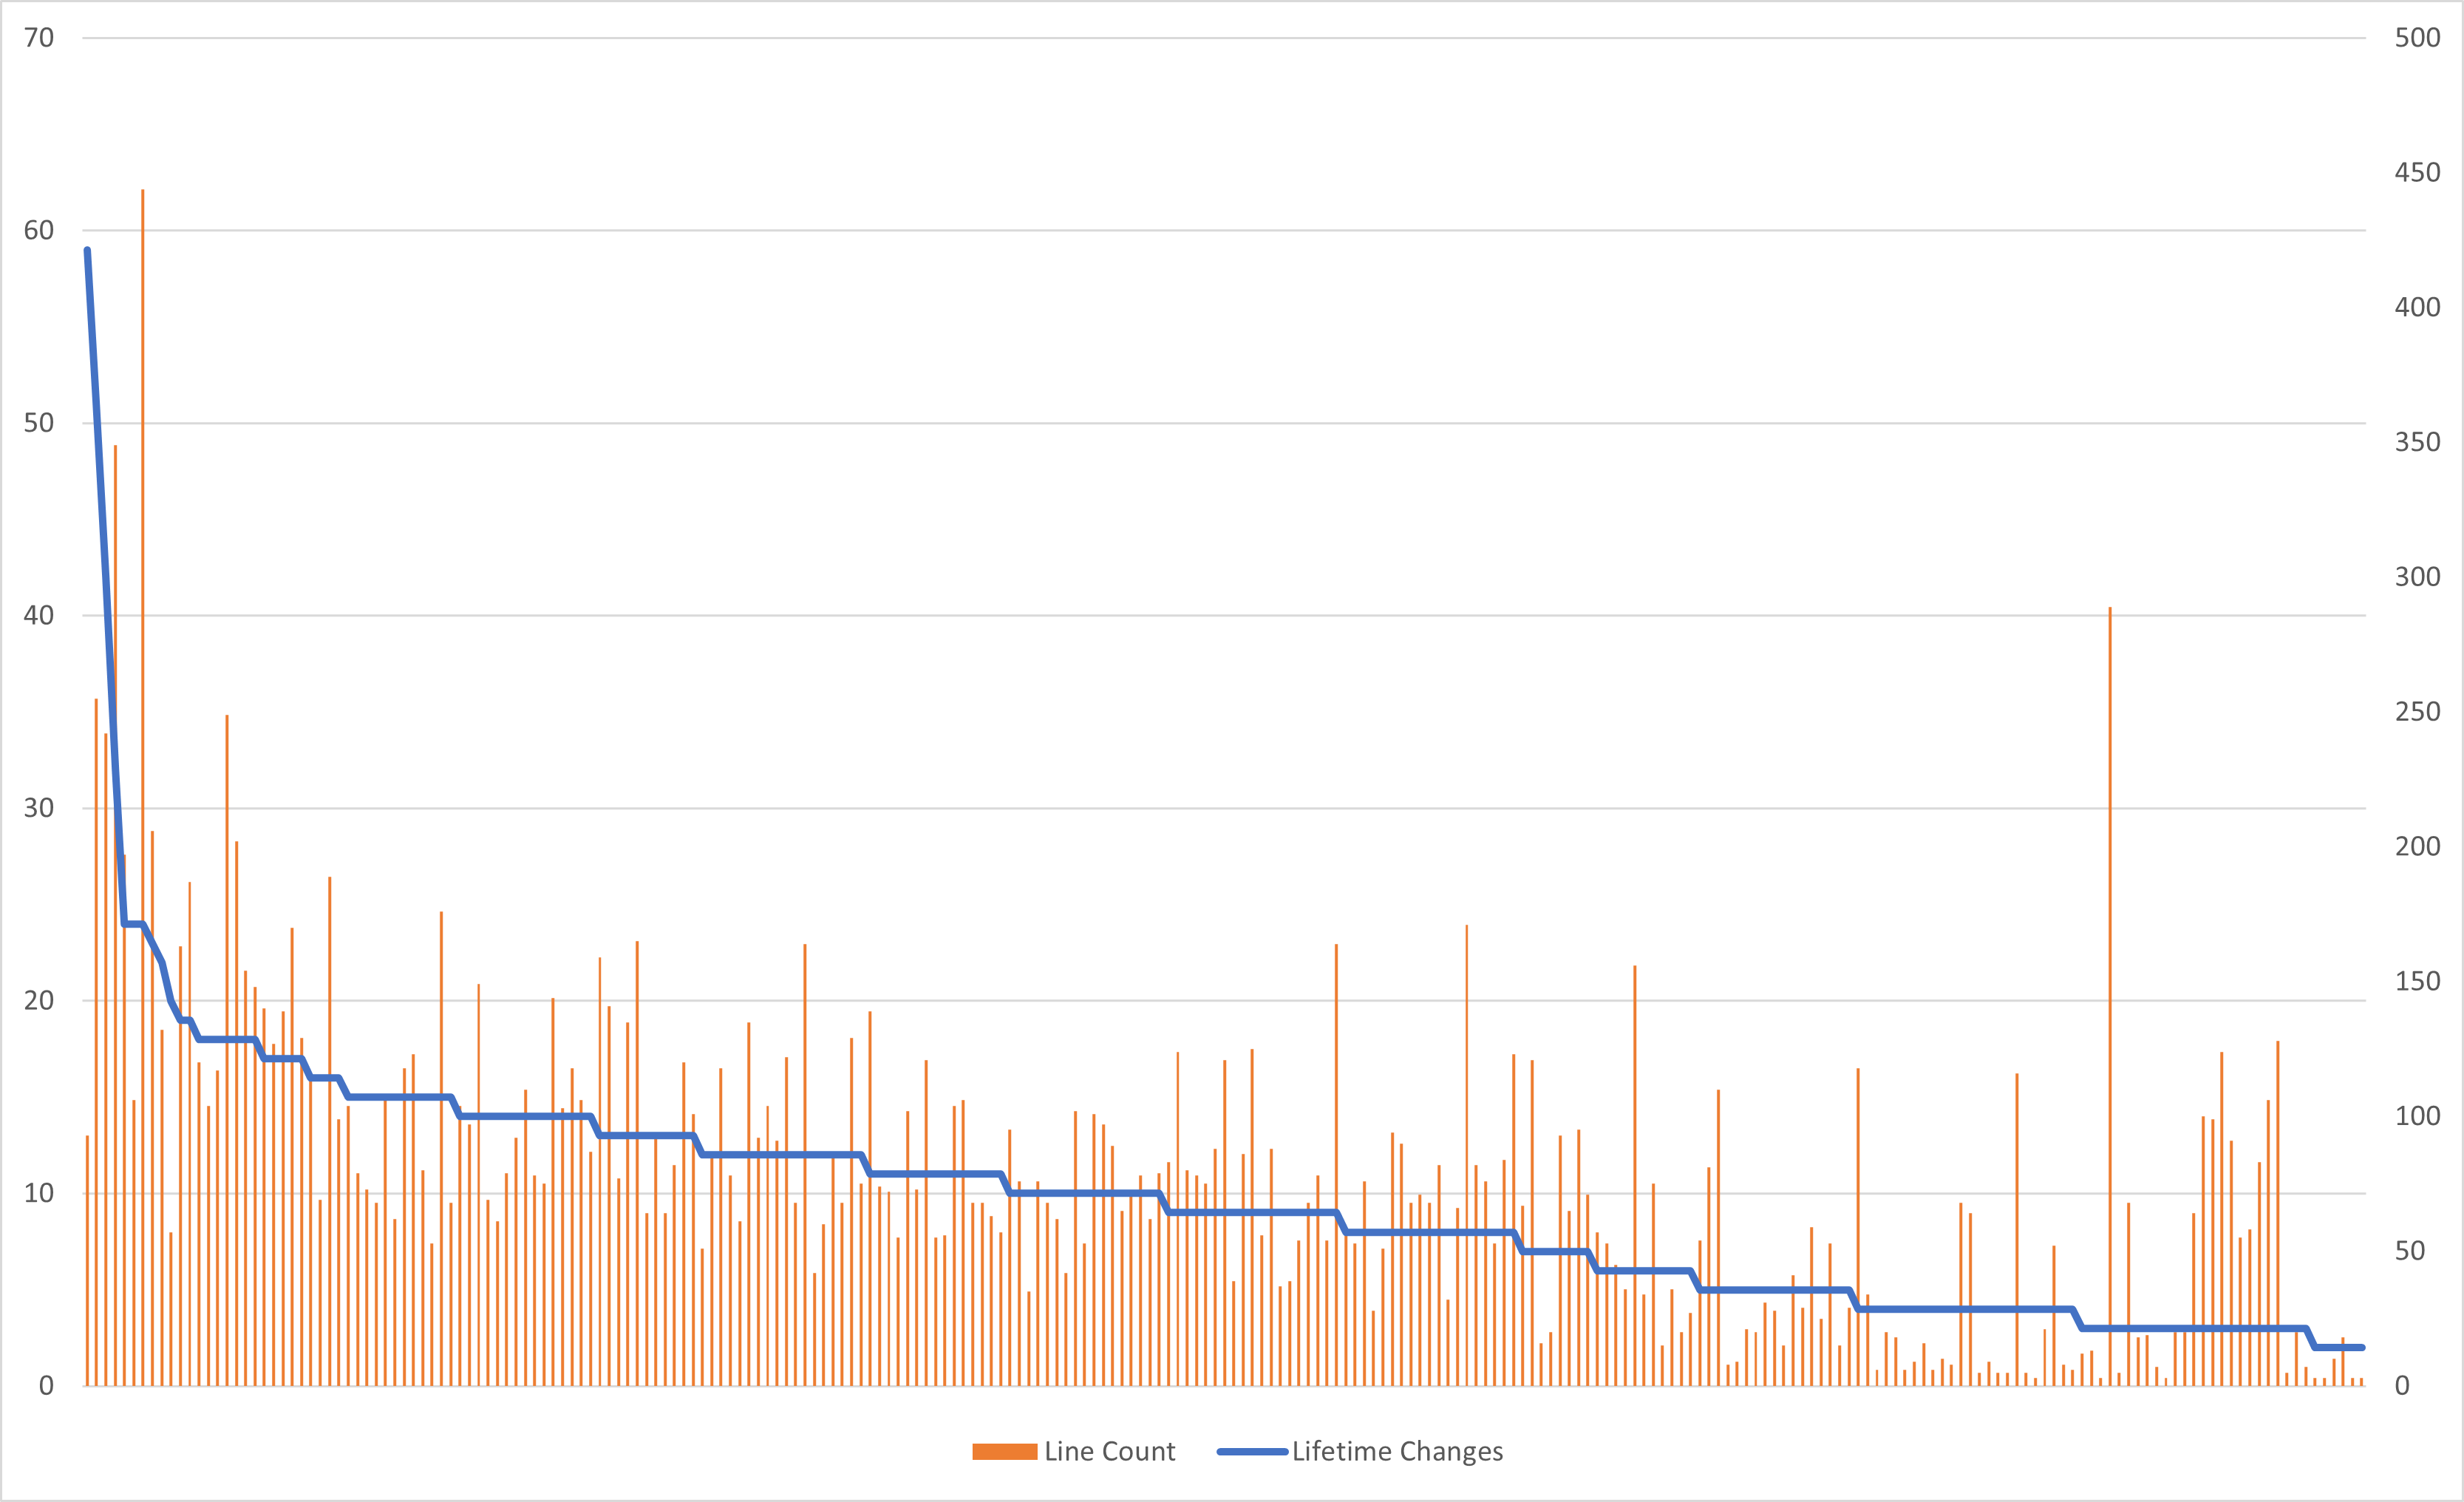
\includegraphics[width=1\textwidth]{images/moment/moment-dev-lines.png}
    \caption{Moment}
    \label{fig:moment-2.10.5-changes}
\end{figure}

\begin{figure}[H]
    \centering
    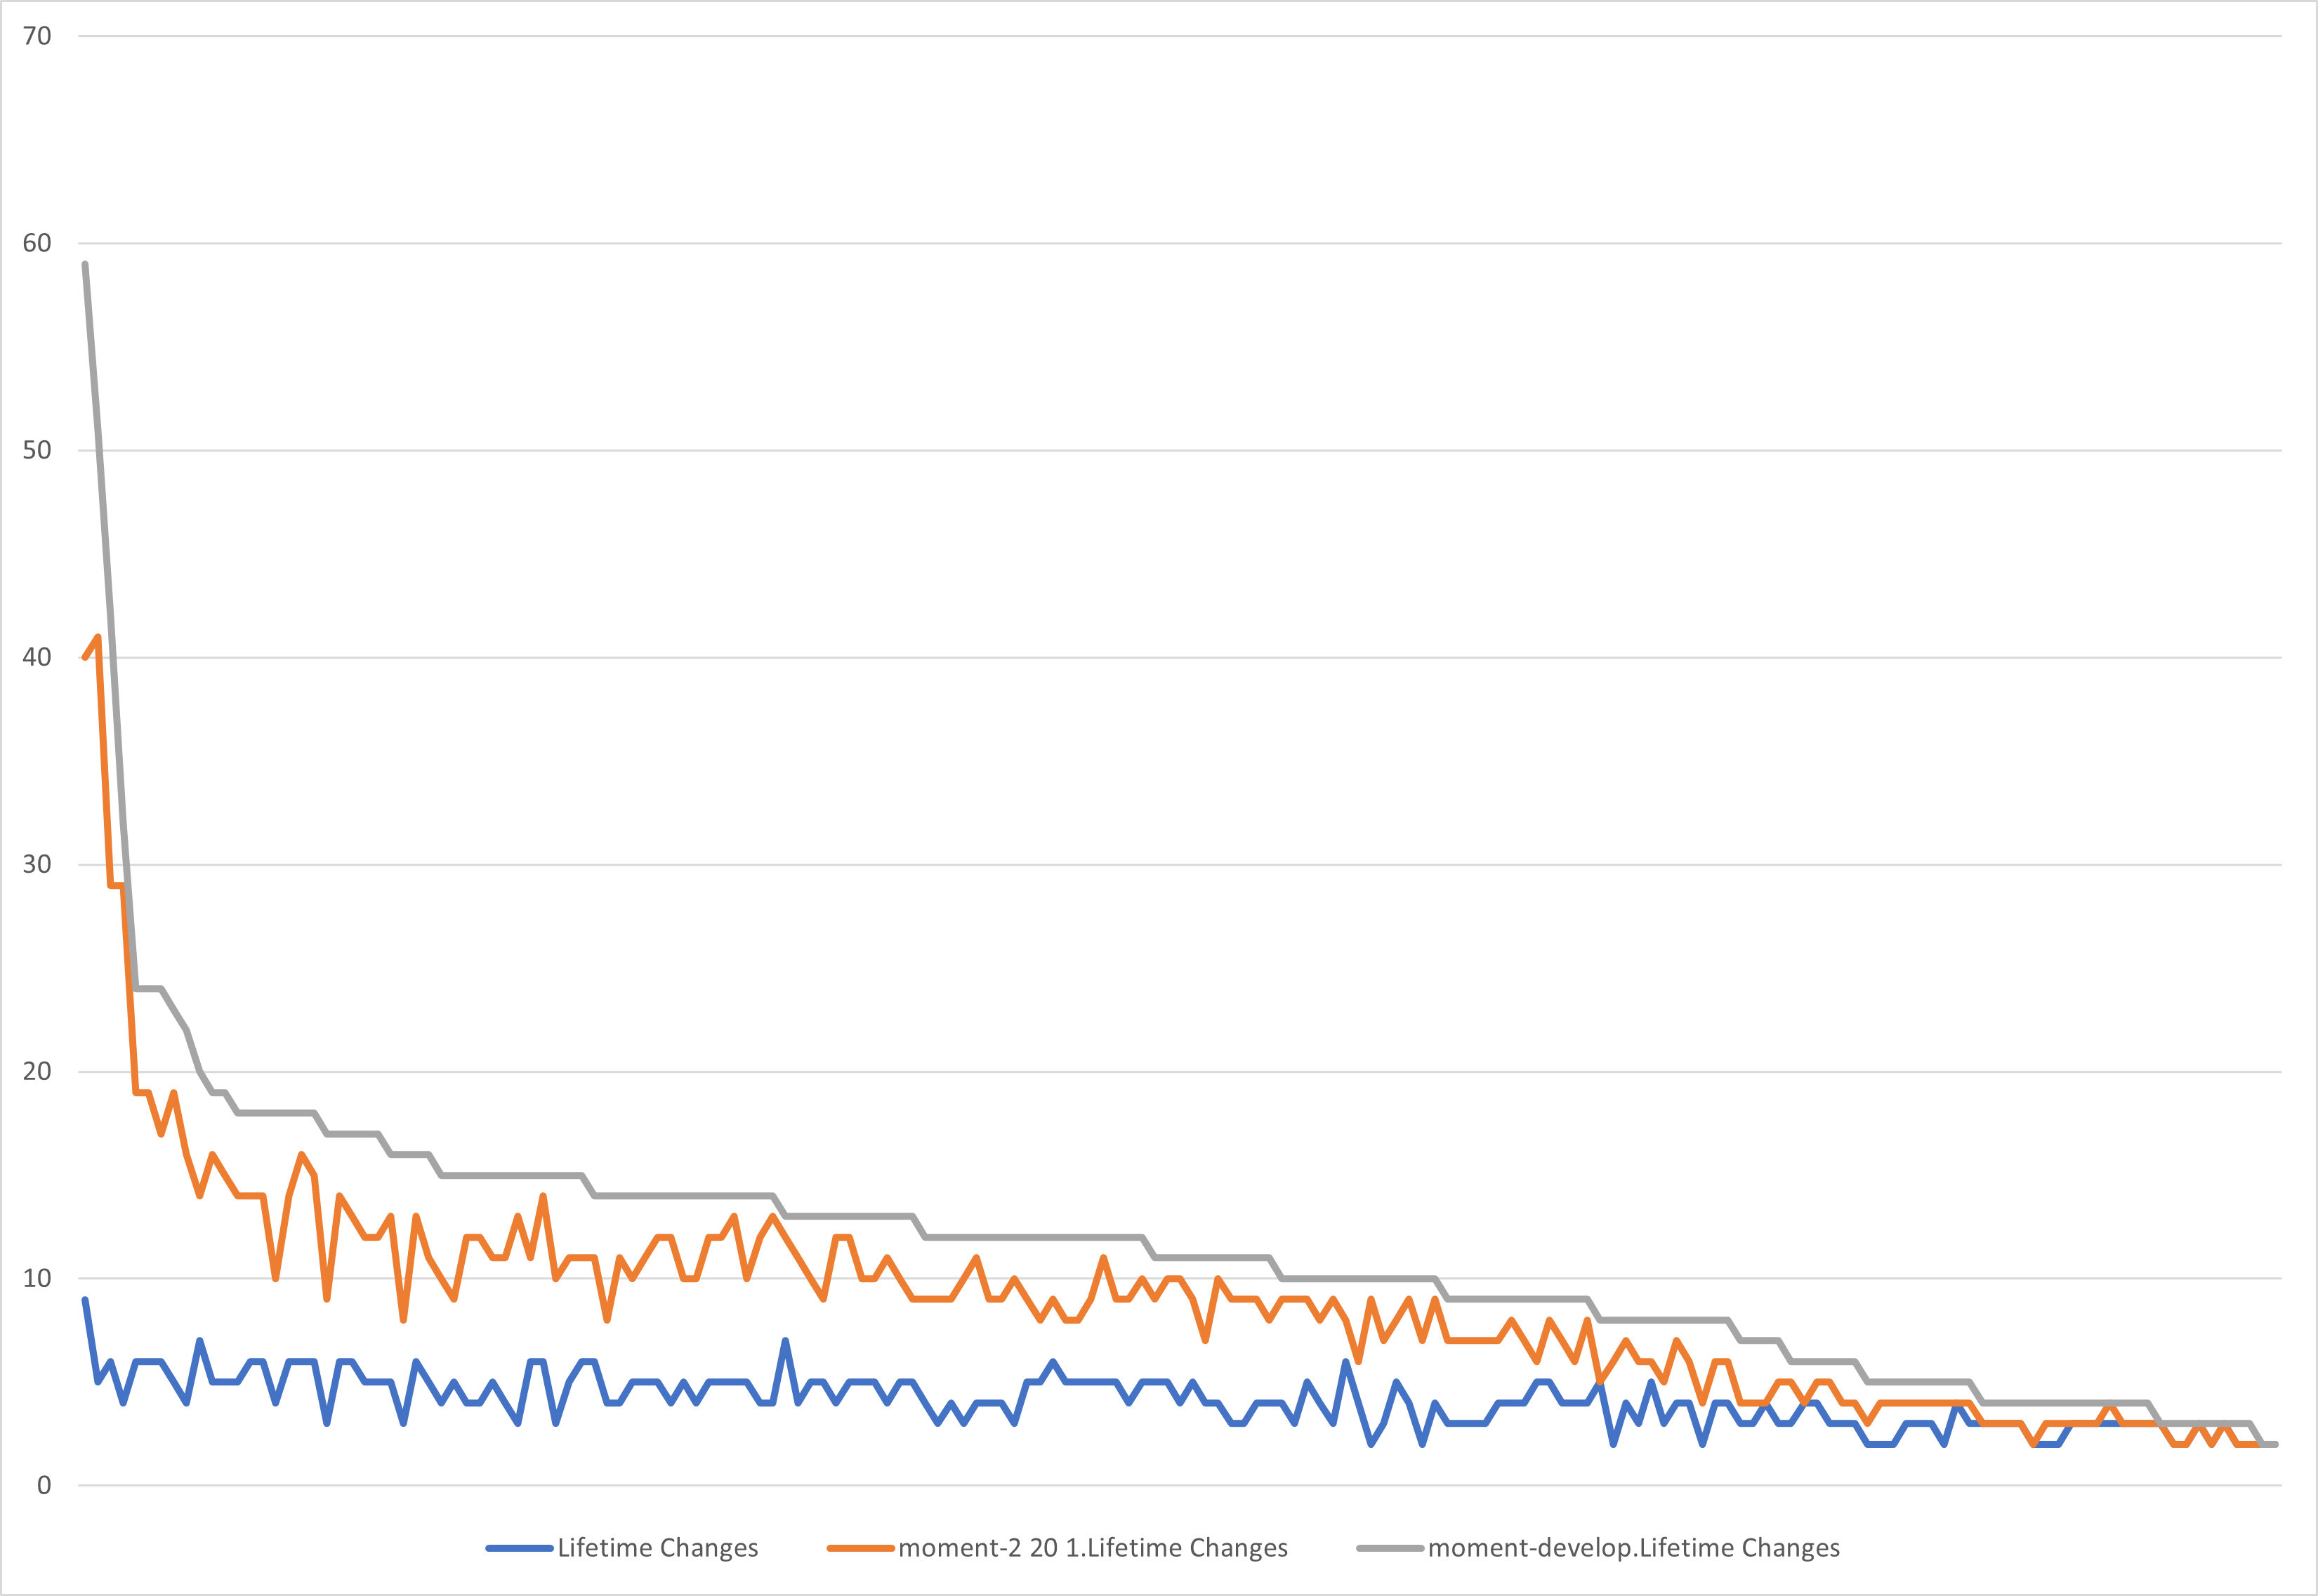
\includegraphics[width=1\textwidth]{images/moment/moment-all-changes.png}
    \caption{Moment}
    \label{fig:moment-2.10.5-changes}
\end{figure}

\subsection{Megfigyelések}